\documentclass[onecolumn, draftclsnofoot,10pt, compsoc]{article}
\usepackage{graphicx}
\usepackage{url}
\usepackage{lscape}
\usepackage{setspace}
\usepackage{parskip}
\usepackage{geometry}
\usepackage{listings}
\usepackage{subfiles}
\usepackage{pdfpages}
\geometry{textheight=9.5in, textwidth=7in}

% 1. Fill in these details
\def \CapstoneTeamName{AgBizClimate}
\def \CapstoneTeamNumber{26}
\def \GroupMemberOne{}%Your Name Here
\def \CapstoneProjectName{ Linking Seasonal Weather Data to AgBizClimate\texttrademark}
\def \CapstoneSponsorCompany{ Oregon State University}
\def \CapstoneSponsorPerson{ Clark Seavert}

% 2. Uncomment the appropriate line below so that the document type works
\def \DocType{		%Software Requirements Document
				%Requirements Document
				%Technology Review
				%Design Document
				Final Document
				}

\newcommand{\NameSigPair}[1]{\par
\makebox[2.75in][r]{#1} \hfil 	\makebox[3.25in]{\makebox[2.25in]{\hrulefill} \hfill		\makebox[.75in]{\hrulefill}}
\par\vspace{-12pt} \textit{\tiny\noindent
\makebox[2.75in]{} \hfil		\makebox[3.25in]{\makebox[2.25in][r]{Signature} \hfill	\makebox[.75in][r]{Date}}}}
% 3. If the document is not to be signed, uncomment the RENEWcommand below
%\renewcommand{\NameSigPair}[1]{#1}

%%%%%%%%%%%%%%%%%%%%%%%%%%%%%%%%%%%%%%%
\begin{document}
\begin{titlepage}
    \pagenumbering{gobble}
    \begin{singlespace}
        \hfill
        % 4. If you have a logo, use this includegraphics command to put it on the coversheet.
        %\includegraphics[height=4cm]{CompanyLogo}
        \par\vspace{.2in}
        \centering
        \scshape{
            \huge CS Capstone \DocType \par
            {\large\today}\par
            \vspace{.5in}
            \textbf{\Huge\CapstoneProjectName}\par
            \vfill
            {\large Prepared for}\par
            \Huge \CapstoneSponsorCompany\par
            \vspace{5pt}
            {\Large\NameSigPair{\CapstoneSponsorPerson}\par}
            {\large Prepared by }\par
            Group\CapstoneTeamNumber\par
            % 5. comment out the line below this one if you do not wish to name your team
            %\CapstoneTeamName\par
            \vspace{5pt}
            {\Large
                \NameSigPair{\GroupMemberOne}\par
            }
            \vspace{20pt}
        }
        \begin{abstract}
			The purpose of this document is to provide documentation regarding the \textit{AgBizClimate} project. We will start off the document by giving a general overview of the \textit{AgBizClimate Project}. This will inclue information about the goals of the project, and information about the project stakeholders. Next we have our requirements document. In this section we will also discuss how our requirements have changed over the last several terms. Next we will be discussing the design document. In this section we will first display our original design document. We will then discuss how our design has changed over the term. After the design document we will display the tech review. Next, we will also display the project poster. Finally we will provide some project documentation regarding how project setup, running the project, how the project works and guids for any API's we are using. After this we will discuss any technical resources for learning more about the technologies that our project uses. Finally, We will end this document with our conclusions and reflections section. This section will involve reflecting on this project and discussing what went well and what didn't go well.\\
        \end{abstract}
    \end{singlespace}
\end{titlepage}
\newpage
\pagenumbering{arabic}
\tableofcontents
% 7. uncomment this (if applicable). Consider adding a page break.
%\listoffigures 
\newpage
%\listoftables
\clearpage

% 8. now you write!
% Will need to review this section to make sure its accurate and that it covers all the bullet points in the 
% requirements for this section.
\section{Introduction}
		\subsection{Purpose}
		This SRS describes the requirements and specifications of the AgBizClimate\texttrademark web application. This document will explain the functional features of this web application. This includes the interface details, design constraints and considerations such as performance characteristics. This SRS is intended to outline how we will proceed with the development of the \textit{AgBizClimate} system.\\

		\subsection{Scope}
			This project is a part of a much larger AgBiz Logic\texttrademark program. However, the purpose of this project is to add a short term climate tool to the \textit{AgBizClimate} module. This limits the scope of the project to the \textit{AgBizClimate} Module. Additionally, we will only be adding the short term climate data tool as the long term climate data tool already exists.\\

		\subsection{Definitions, Acronyms and Abbreviations}
			REST - Representation State Transfer, This is a type of architecture that manages preforms operations on the state of the program. This is especially popular in web development.\\
			API- Application Programming Interface. This is a piece of software that allows a connection to another piece of software providing some sort of service.\\
			Thredds Data Server - This is a web server that provides meta-data and data access for scientific data sets using OPeNDAP along with some other remote data access protocols.\\
			OPeNDAP - Open-source Project for a Network Data Access Protocol. This is the protocol we will be using to retrieve the data sets from the Thredds data server.\\
			NMME - North American Multi-Model Ensemble. This is a data set that brings together a variety of different weather models into one data set.\\
			Climate Scenario - This is a theoretical calculation of yields, inputs and of the overall budget for one situation based on the climate data.\\
			NETCDF - This is a file storage format for large scientific data sets especially good for any data that is referenced on a grid and related to is geo-location.\\
			SQL Database - This is a relational database that makes storing and accessing data easy.\\
			Container - A virtualized operating system that is used to host and deploy web development projects. This allows projects to be easily portable between different operating systems and platforms.\\
			Mount Bind - This is the practice of mounting a directory from the native os to the container such that if either the container or the native operating system. This allows changes in the files to be reflected in both the container and the native operating system.\\
			

			\renewcommand\refname{\vskip -1cm}
		\subsection{References}

		\nocite{*}
    \bibliographystyle{IEEEtran}
    \bibliography{IEEEabrv,References}


		\subsection{Overview}
			Seasonal climate is one of the essential factors that affects agricultural production. As a module of \textit{AgBiz Logic}, \textit{AgBizClimate} delivers essential information about climate change to farmers, and help professionals to develop management pathways that best fit their operations under a changing climate. This project aims to link the seasonal climate data from the NMME data set to \textit{AgBiz Logic} so that it can provide changes in net returns of crop and livestock enterprises through powerful graphics and tables. \\
			Currently \textit{AgBizClimate} has a long-term climate tool but no such tool exists for short term climate data. We will implement a tool to extract short-term climate data from the NMME data set, display it to the user and allow the user to adjust crop and livestock yields or quality of products sold and, production inputs. Moreover, a landing tool will be developed to allow users to switch between short-term seasonal tool and long-term climate data tool.\\
			
	\subsection {Product Functions}
				\textit{AgBizClimate} is a web based decision tool that will allow users to gain specific insight on how localized climate data for the next seven months will affect their crop and livestock yields or quality of products sold and production inputs. The \textit{AgBizClimate} tool will allow users to input their location (state, county) and a budget for the specific crop or livestock enterprise. \textit{AgBizClimate} will select climate data for the next seven months for that location and provide graphical data showing temperature and precipitation. Users will then be able to change yields or quality of product sold by a percentage they think these factors will affect and modify production inputs. Finally the tool will calculate the net returns.\\

	\subsection{User Characteristics}
		\textit{AgBizClimate} users can be split into two subgroups, agricultural producers and climate researchers. The first subgroup, agricultural users who use this product tend to be between fifty and sixty years old of mixed gender. Their educational background ranges from high school to the completion of college. The primary language this group uses is English, but there are some Spanish users as well. Most of the users in this group tend to have novice computational skills. The primary domain for these users is agricultural and business management. Most agricultural producers who use this product are motivated by the potential profit that the decision tool \textit{AgBizClimate} could potentially offer. The second subgroup, climate researchers range from ages twenty to forty and are of mixed gender. The educational background for most climate researchers  exceed the postgraduate level with their primary language being English. These users generally have advanced computational skills and are motivated by the easily accessible climate and weather data.\\

	\subsection{Constraints}
		There are several key constraints that this product has to work within. Firstly, We are limited by the availability and completeness of the data from the NMME data set. The NMME Data set does not have data for every point on in the country. Secondly, we must use the Threadds server hosted by University of Idaho to get the data in the NetCDF format. The tooling provides a variety of access methods however, the only method that currently works is downloading the whole file. Fourthly, we don’t have access to any of the hardware that \textit{AgBizClimate} is exists on as it is being managed by a third party. This will prevent us from improving the hardware or cause roadblocks if their servers are having issues. Lastly, we are limited to using the languages Python and JavaScript since we are integrating our product into an already existing project.\\

	\subsection {Assumptions and Dependencies}
		We are assuming that the NMME Thredds data base will allow us to pull location based temperature and precipitation data. This data will come in the form of a NetCDF files which we will then read and format a JSON response. Due to the fact that we are writing an addition to an existing project we do not need to interact with the user budgets as these have already been defined. This fact extends to the calculations portion of the \textit{AgBizClimate} product. Our team will simply be accessing data via the NMME threadds database, will then format the data, store the data, and hand the data over to the front end or some other sort of client.\\


\section{Requirements Document}
    \subsection{Original Document}
        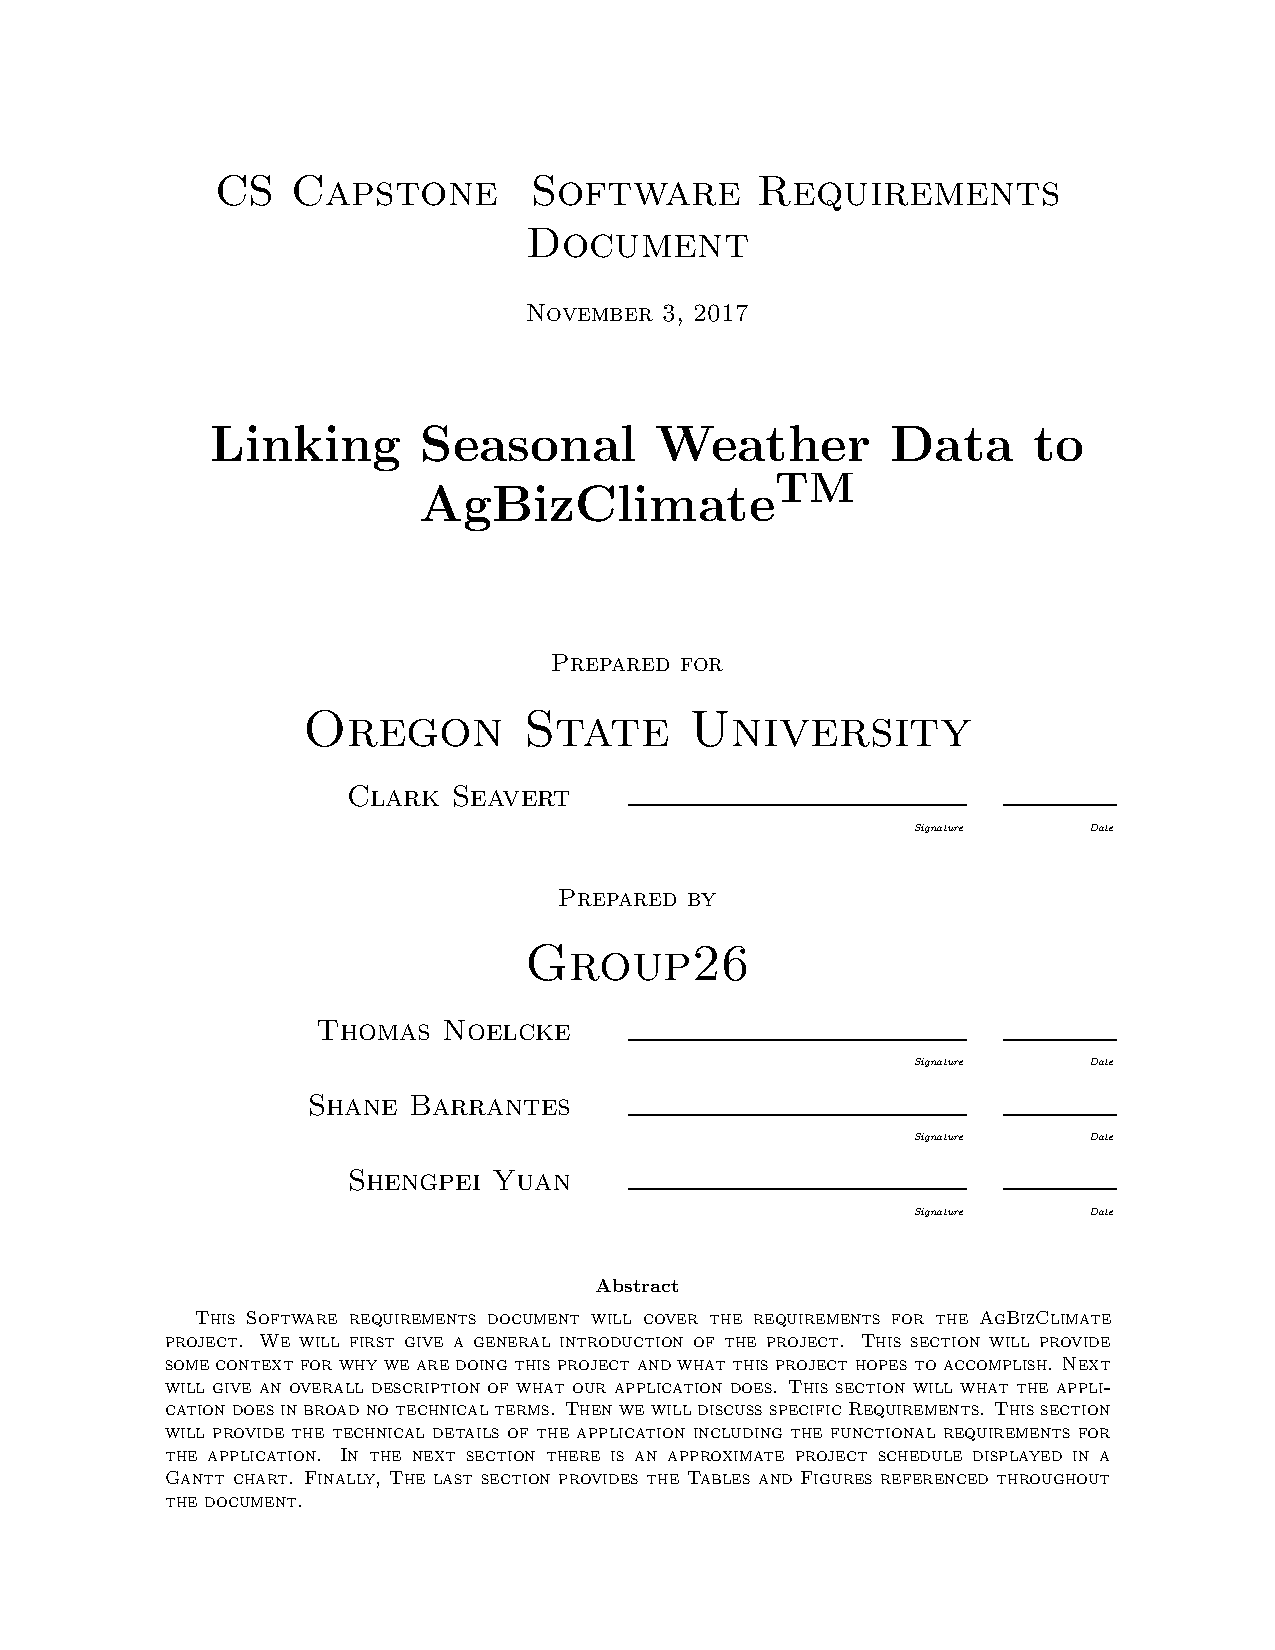
\includepdf[pages={1-16}]{./Original-Docs/Requirements-Document-Original/AgBizClimateSRS.pdf}
    
    \subsection{Changes}
\section{Design Document}
    \subsection{Original Document}
        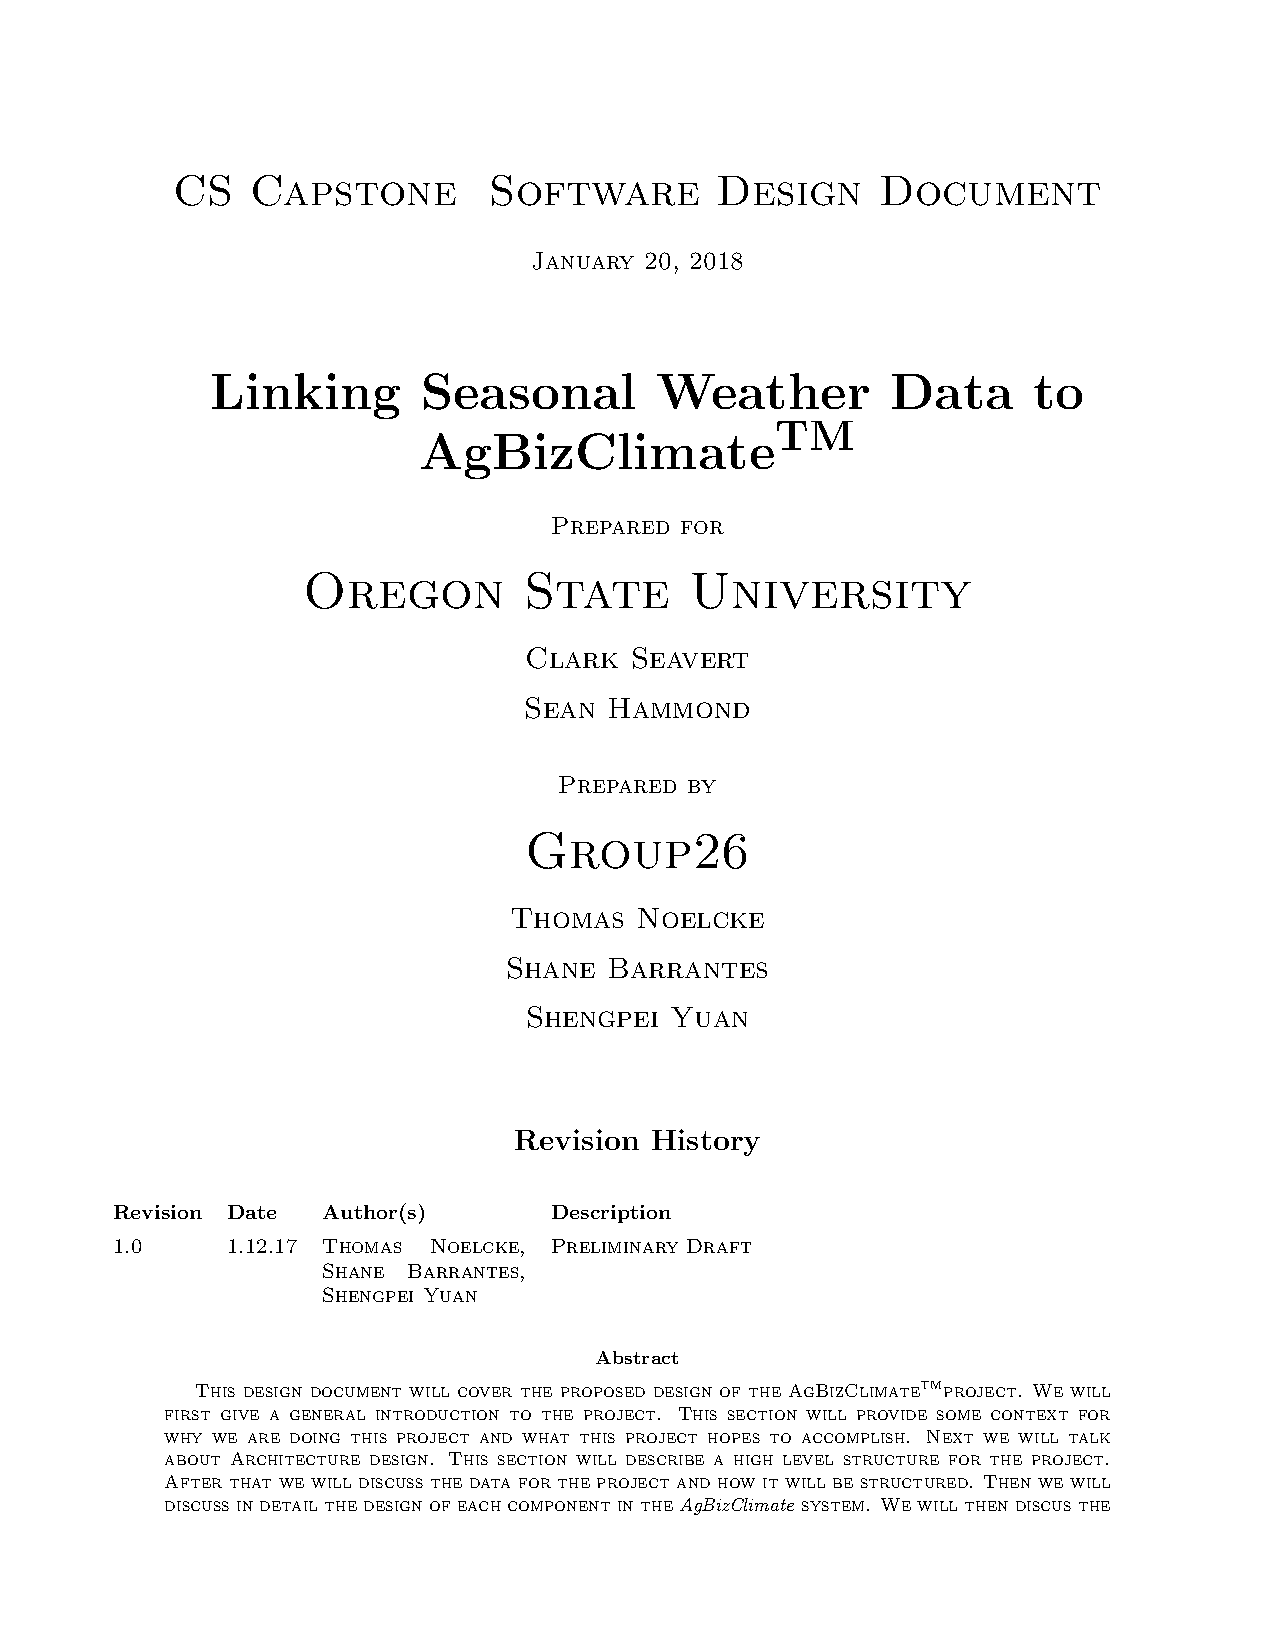
\includepdf[pages={1-33}]{./Original-Docs/DesignDoc/AgBizClimateDesignDoc.pdf}
    \subsection{Changes}
		
		
\section{Tech Review}
	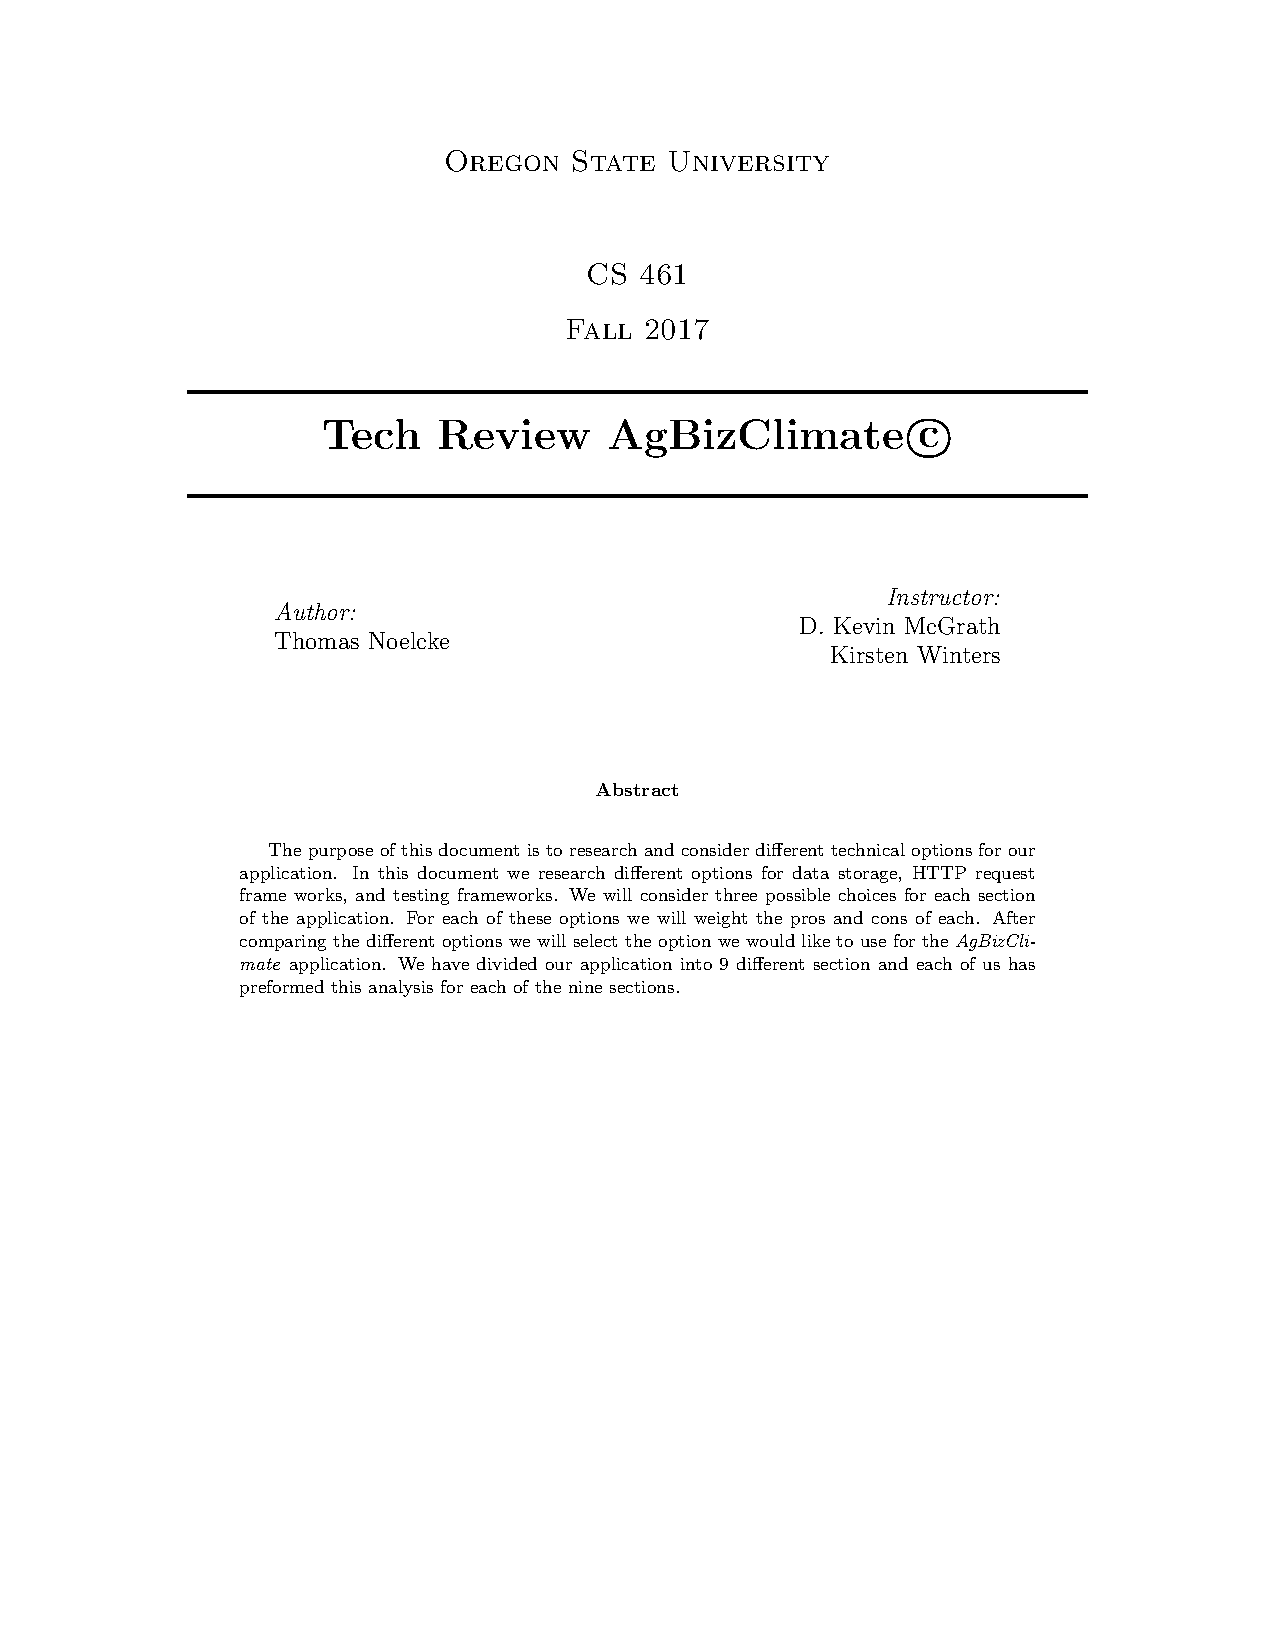
\includepdf[pages={1-23}]{./Original-Docs/Tech-Review/TechReviewCombined.pdf}

\section{Weekly Blog Posts}
    \subsection{Shane Barrantes}
    
    \subsection{Thomas Noelcke}
        In this section Will be every weekly update that I've made through out the term. It should be noted that I will denote the weeks by [term number].[week] where the week is the week number in the respective term and the term number represents the term. There will be 3 terms 1, 2 and 3 which will represent fall winter and spring respectively.\\ 
        
        
        
    
    \subsection{Shengpei Yuan}

\section{Final Poster}

%We will put set up and configuration steps here. We will also discuss how our project works. Hardware and software requirements. User guids, API Docs.
\section{Project Documentation}
    \subsection{Essential Documents}
    
    \subsection{Recommended Technical Resources}

\section{Conclusions and Reflections}
    \subsection{Shane Barrantes}
    
    \subsection{Thomas Noelcke}
    \subsubsection {Week 1.1}
        In this week our group had not yet been formed. As such there is no report for this week.
    \subsubsection{Week 2.1}
		
		    \paragraph{Plans:} \hfill \break
		    
		    \begin{itemize}
		        \item Set Up First Group Meeting
		        \item Meet With Client
		        \item Work On Problem Statement
		    \end{itemize}
		
		    \paragraph{Problems:} \hfill \break
		    
		    \begin{itemize}
		        \item Group Communication 
		    \end{itemize}
		    
		    \paragraph{Progress:} \hfill \break
		    \begin{itemize}
		        \item Started Slack Channel with group 10/4
		        \item Contacted Client 10/4
		        \item met with group 10/5
		        \item setup meeting with client for 10/10 on 10/5
		        \item set up meeting with lead developer for 10/12 on 10/6
		    \end{itemize}
		    
		    \paragraph{Summary} \hfill \break
		         This week our group started to get organized and reached out to our client. We also had a group meeting where we briefly discussed project details along with what skill sets we had. We also had a discussion about group communication.\\
		         
		\subsubsection{Week 1.3}
		
		    \paragraph{Plans:} \hfill \break
		        
		        \begin{itemize}
		            \item Meet with Client
		            \item Create Problem Statement Rough draft
		            \item start working on requirements document
		            \item Technical meeting with Sean Hammond
		        \end{itemize}
		        
		    \paragraph{Problems:} \hfill \break
		    
		    \begin{itemize}
		        \item We don't know how the NWCTB interface will work as we don't have API Access yet.
		    \end{itemize}
		
		    \paragraph{Progress:} \hfill \break

		    \begin{itemize}
		        \item Finished Rough Draft of Problem Statement 10/9
		        \item Met with Clark on 10/10
		        \item Met with Seen Hammond on 10/12
		    \end{itemize}
		    
		    \paragraph{Summary:} \hfill \break
		    	This week we met with Clark and Sean to start the conversation about our project. The first meeting with Clark was a higher level overview of our project where the second meeting with Sean was a technical meeting where we discussed the technical details of the project. We found one major blocker moving forward which is we don't have NWCTB API Access. To design our project we will need to figure this out.\\ 
		        
		\subsubsection{Week 4.1}
		
		    \paragraph{Plans:} \hfill \break
		        
		        \begin{itemize}
		            \item Turn in final drafts for individual problem statements
		            \item Start working on Requirements Document
		            \item Work with group to start compiling group problem statement
		            \item Try to get NWCTB API Access
		        \end{itemize}
		        
		    \paragraph{Problems:} \hfill \break
		        
		        \begin{itemize}
		            \item We Still don't have NWCTB API Access.
		        \end{itemize}
		        
		    \paragraph{Progress:} \hfill \break
		    
		        \begin{itemize}
		            \item Met as a group to work on the group problem statement 10/18
		            \item Finalized and turned in the group problem statement 10/19
		            \item Followed up with Clark regarding setting up a meeting with the Northwest Climate Toolbox to gain API Access
		        \end{itemize}
		        
		        \paragraph{Summary:}
		            This week we worked as a group to get our problem statement finalized. We also followed up with Clark regarding setting up a meeting with the Northwest Climate toolbox as this is the major blocker for our project. Finally, we sent our final group problem statement off to Clark for final approval. Clark approved our problem statement and we turned it in. This week we also started to think about our requirements list and what we will need to do next week to get started on our requirements document.\\
		    
		\subsubsection{Week 5.1}
			\paragraph{Plans:} \hfill \break
		        
		        \begin{itemize}
		            \item Set up meeting with NWCTB
		            \item Start requirements document
		            \item line requirements document
		            \item Turn in rough draft of requirements document
		        \end{itemize}
		        
		    \paragraph{Problems:} \hfill \break
		        \begin{itemize}
		            \item We still don't have NWCTB API Access
		        \end{itemize}
		
		    \paragraph{Progress:} \hfill \break
		    
		    \begin{itemize}
		        \item Set up meeting to discuss requirements document for 10/24 on 10/23
		        \item Started requirements document outline 10/23
		        \item Finished First rough draft of requirements document 10/27
		        \item Turned In rough draft of requirements document 10/27
		        \item Meet as group with TA to review this weeks progress 10/27
		        \item Meet as a group to discuss progress on requirements document 10/27
		    \end{itemize}
		    
		    \paragraph{Summary:}
		        
		        This week we started off the week meeting with our Clients lead developer to start drafting our requirements document. The purpose of this meeting was to direct our efforts on writing the requirements document. This meeting was a great help and helped us to get a good start on the document.  We also met with the TA on Friday and discussed our progress this week. After our meeting with the TA we meet as a group to go over our progress on the requirements document and to plan for next week.\\
		
		\subsubsection{Week 1.6}
		
		    \paragraph{Plans:} \hfill \break
		        
		        \begin{itemize}
		            \item Meet with Client to review draft of requirements document
		            \item work with group to finish SRS final draft.
		            \item follow up with Clark about setting up meeting for NWCTB API Access.
		        \end{itemize}
		
		    \paragraph{Problems:} \hfill \break
		        
		        \begin{itemize}
		            \item Still don't have API Access for NWCTB
		        \end{itemize}
		        
		    \paragraph{Progress:} \hfill \break
		    
		        \begin{itemize}
		            \item Worked on SRS 10/30
		            \item Met with client to review SRS progress 10/31
		            \item worked on SRS 10/31
		            \item Worked on SRS 11/1
		            \item Worked on SRS 11/2
		            \item Worked on SRS 11/3
		            \item Turned in SRS 11/3
		        \end{itemize}
		
		    \paragraph{Summary:} \hfill \break
		        This week we met with our client to go over our draft of our SRS. During this meeting he suggested some edits that we made the following day. Additionally, we also worked as a group on completing our SRS. We currently have the final draft done but are doing a final proof read before we turn it in this evening.\\
		
		\subsubsection{Week 1.7}
		
		    \paragraph{Plans:} \hfill \break
		        \begin{itemize}
		            \item Divide Project up into 9 distinct parts for tech review.
		            \item Start working on tech review
		            \item Follow up with Clark regarding NWCTB API Access
		        \end{itemize}
		
		    \paragraph{Problems:} \hfill \break
		        \begin{itemize}
		            \item Still don't have NWCTB API Access
		            \item Beginning to notice we are not making progress on API Issue.
		        \end{itemize}
		
		    \paragraph{Progress:} \hfill \break
		        \begin{itemize}
		            \item Divided project into 9 parts 11/8
		            \item worked on rough draft of tech review 11/12
		        \end{itemize}
		        
		    \paragraph{Summary:} \hfill \break
		        This week we divided up the project into 9 different parts so each group members could each have three parts. We then picked the parts of application that we wanted to review. After that we then got working on the tech review rough draft.\\
		
		\subsubsection{Week 1.8}
		
			\paragraph{Plans:} \hfill \break
			    \begin{itemize}
			        \item finish tech review
			        \item set up meeting with Clark and Sean for design document.
			        \item Meet up and discuss tech review and peer review each others tech review
			    \end{itemize}
		
		    \paragraph{Problems:} \hfill \break
		        \begin{itemize}
		            \item NWCTB Still hasn't responded to our request for API access
		        \end{itemize}
		
		    \paragraph{Progress:} \hfill \break
		        \begin{itemize}
		            \item worked on tech review 11/13
		            \item set up meeting with Clark and Sean on 11/13 for 11/21 for design document
		            \item Preformed peer review in class on tech review 11/14
		            \item Shengpei and I met up to review each others tech review 11/16
		        \end{itemize}
		        \paragraph{Summary:}
		             This week we continued to work on our tech reviews. These documents are nearly complete. Some group members met to discuss the structure and content of the tech review. We will be ready to turn in our tech review next Tuesday. Additionally we set up a meeting with Clark and Sean to review the tech review.\\
		    
		\subsubsection{Week 1.9}
		
			\paragraph{Plans:} \hfill \break
                \begin{itemize}
                    \item Meet with Clark and Sean to go over the design document
                    \item finalize drafts of tech review
                    \item start design document
                \end{itemize}		
		
		    \paragraph{Problems:} \hfill \break
		        \begin{itemize}
		            \item Still haven't heard back from NWCTB regarding API access.
		        \end{itemize}
		
		    \paragraph{Progress:} \hfill \break
		        \begin{itemize}
		            \item Worked on tech review 11/20
		            \item Did a final review with Shengpei 11/20
		            \item We meet with Sean on 11/21 at 1:30 PM
		            \item discussed API access with Sean at our meeting 11/21.
		            \item finished Tech review 11/21
		            \item Started work on design document 11/24
		        \end{itemize}
		        
		    \paragraph{Summary:} \hfill \break
		         This week we finished up our tech reviews. I helped Shengpei finish up his tech review on Monday. I finished up my tech review Tuesday evening. Additionally, We also met with Seen Hammond to discuss our design document. We also started our design document on 11/24/2017.\\
		
		\subsubsection{Week 1.10}
		
		    \paragraph{Plans:} \hfill \break
		        \begin{itemize}
		            \item Finish Design Document
		            \item Start Progress Report
		            \item Research alternatives to NWCTB
		        \end{itemize}
		
		    \paragraph{Problems:} \hfill \break
		        \begin{itemize}
		            \item Still don't have NWCTB API Access.
		        \end{itemize}
		
		    \paragraph{Progress:} \hfill \break
		        \begin{itemize}
		            \item Worked on Design Document 11/26 - 12/1
		            \item Submitted rough draft of design document to Sean Hammond and Clark Seavert 11/30.
		            \item Started working on progress report 12/1.
		            \item Researched alternatives to NWCTB 12/1.
		        \end{itemize}
		        
		      \paragraph{Summary:} \hfill \break
		        This week was busy week for our project. This week we worked on the design document. Currently we are nearly completed with the design document and will be able to finish up the document before EOD today. This week we also started working on the progress report. We outlined the report and will start working on the doc as soon as we are done with the design doc. We will also need to produce content for the presentation we are going to get together and give on Sunday evening.\\
		
		    
    \subsection{Shengpei Yuan}

\section{Appendix}    

    \subsection{Appendix 1: Essential Code Listings}

    \subsection{Appendix 2: Catch all}
\end{document}
